\chapter{Операторные методы в квантовой механике. Метод вторичного квантования}

\section{Операторы уничтожения и рождения в теории линейного гармонического осциллятора} \footnote{<<Линейность>> осциллятора понимается в приближении одномерных малых колебаний вблизи положения равновесия}

\begin{equation}
\label{eq:7_1_1}
\underbrace { \brc{ \frac{\op{p_x}^2}{2m} + \frac{m\omega^2 \op{x}^2}{2} } }_{\text{гамильтониан ГО}} \ket{n} = E_n \ket{n}
\end{equation}

Введём обозначения:
$$
\begin{gathered}
\op{\xi} = \frac{\op{x}}{a_0} = \sqrt{\frac{m\omega}{\hbar}} \op{x} \\
\op{p}_{\xi} = \frac{\op{p_x}}{p_0} = \frac{1}{\sqrt{m\hbar \omega}} \op{p_x}
\end{gathered}
$$

Здесь были введены \textbf{осцилляторные единицы} длины и импульса:
$$
\begin{gathered}
a_0 = \sqrt{\frac{\hbar}{m\omega}} \\
p_0 = \frac{\hbar}{a_0} = \sqrt{m\hbar \omega}
\end{gathered}
$$

Поделим \eqref{eq:7_1_1} на осцилляторную единицу энергии $\hbar \omega$:

$$
\underbrace{ \frac{1}{2} \brc{ \op{p_\xi}^2 + \op{\xi}^2} }_{\mathclap{\op{h}~\text{-- безразмерный гамильтониан}}} \ket{n} = \epsilon_n \ket{n},~~~ \text{где}~~ \epsilon_n = \frac{E_n}{\hbar \omega}
$$

\begin{equation}
\label{eq:7_1_2}
\brs{\op{\xi}, \op{p}_\xi} = \frac{1}{\hbar} \brs{\op{x}, \op{p}_x} = i
\end{equation}

Введём эрмитово сопряжённые \textbf{(но не эрмитовые!)} операторы:
$$
\left\{
\begin{aligned}
\op{a} \equiv \frac{\op{\xi} + i\op{p_\xi}}{\sqrt{2}} \\
\op{a}^\dag \equiv \frac{\op{\xi} - i\op{p}_\xi}{\sqrt{2}}
\end{aligned}
\right. ~~~ \Rightarrow ~~~ \left\{
\begin{aligned}
\op{\xi} = \frac{\op{a} + \op{a}^\dag}{\sqrt{2}} \\
\op{p}_\xi = \frac{\op{a} - \op{a}^\dag}{\sqrt{2}} \\
\end{aligned} \right.
$$

Перепишем гамильтониан через $\ann$ и $\cre$:
$$
\cre\ann = \frac{1}{2} (\op{\xi} - i\op{p_\xi})(\op{\xi} + i\op{p_\xi}) = \left. \frac{1}{2}(\op{\xi}^2 + \op{p_\xi}^2 + i \brs{\op{\xi}, \op{p_\xi}}) \right|_{\text{\eqref{eq:7_1_2}}} = \frac{1}{2} (\op{\xi}^2 + \op{p_\xi}^2 - 1) \equiv \op{h} - \frac{1}{2}
$$

$$
\op{h} = \cre\ann + \frac{1}{2}
$$

\begin{equation}
\label{eq:7_1_3}
\op{h} \ket{n} = \epsilon_n \ket{n}
\end{equation}

\section{Энергетрический спектр линейного гармонического осциллятора.}

$$
\brs{\ann, \cre} = \frac{1}{2} \brs{ \op{\xi} + i\op{p_\xi},  \xi - i\op{p_\xi}} = \frac{1}{2} \brc{ i\brs{\op{p_\xi}, \op{\xi}} - i \brs{\op{\xi}, \op{p_\xi}} } = -\frac{2i}{2} \underbrace{ \brs{\op{\xi}, \op{p_\xi}}}_{= i} = 1
$$

\begin{equation}
\label{eq:7_2_1}
\brs{\ann, \cre} = 1
\end{equation}

Используя тождество $[\op{A}, \op{B}\op{C}] = [\op{A}, \op{B}] \op{C} + \op{B} [\op{A}, \op{C}]$, получим:

\begin{equation}
\label{eq:7_2_2}
\brs{\cre, \op{h}} = \brs{\cre, \cre\ann} = \underbrace{\brs{\cre, \cre}}_{= 0} \ann + \cre \underbrace{\brs{\cre, \ann}}_{= -1} = - \cre
\end{equation}

\begin{equation}
\label{eq:7_2_3}
\brs{\ann, \op{h}} = \brs{\ann, \cre\ann} = \underbrace{\brs{\ann, \cre}}_{= 1} \ann + \cre \underbrace{\brs{\ann, \ann}}_{= 0} = \ann
\end{equation}

Домножим \eqref{eq:7_1_3} на $\cre$:
$$
\cre \op{h} \ket{n} = \epsilon_n \cre \ket{n}
$$

Из \eqref{eq:7_2_2}:
\begin{equation}
\label{eq:7_2_4}
\op{h} \brc{\cre \ket{n}} = (\epsilon_n + 1)(\cre \ket{n})
\end{equation}

$(\cre \ket{n})$ -- собственный вектор гамильтониана $\op{h}$ с собственным значением $(\epsilon_n + 1)$

Из \eqref{eq:7_1_3} и \eqref{eq:7_2_4} введём обозначения:
\begin{equation}
\label{eq:7_2_5}
\left[
\begin{aligned}
\epsilon_{n+1} \equiv \epsilon_n + 1 \\
\cre \ket{n} \equiv c_n \ket{n+1}
\end{aligned}
\right.
\end{equation}

$\cre$ обычно называют \textbf{оператором рождения} (повышения) кванта колебаний (увеличивает квантовое число на единицу)

\begin{equation}
\label{eq:7_2_6}
\abs{c_n}^2 = \bk{\cre n}{\cre n} = \left. \bfk{n}{\ann\cre}{n} \right|_{\text{\eqref{eq:7_2_1}}} = \bfk{n}{\cre\ann + 1}{n} = \bfkh{n}{\op{h} + \frac{1}{2}}{n} = \epsilon_n + \frac{1}{2}
\end{equation}

Домножим \eqref{eq:7_1_3} на $\ann$:
$$
\ann\op{h} \ket{n} = \epsilon_n \ann \ket{n}
$$

Из \eqref{eq:7_2_3}:
\begin{equation}
\label{eq:7_2_7}
\op{h}(\ann\ket{n}) = (\epsilon_n - 1)(\ann \ket{n})
\end{equation}

Т.е. $(\ann\ket{n})$ -- собственный вектор гамильтониана $\op{h}$, отвечающий собственному значению $(\epsilon_n - 1)$.

Введём обозначения:
\begin{equation}
\label{eq:7_2_8}
\left[
\begin{aligned}
\epsilon_{n-1} \equiv \epsilon_n - 1 \\
\ann \ket{n} = c_{n}' \ket{n-1}
\end{aligned}
\right.
\end{equation}

$\ann$ -- \textbf{оператор уничтожения} кванта колебаний.

\begin{equation}
\label{eq:7_2_9}
\abs{c_n'}^2 = \bk{\ann n}{\ann n} = \bfk{n}{\cre\ann}{n} = \bfkh{n}{\hbar - \frac{1}{2}}{n} = \epsilon_n - \frac{1}{2}
\end{equation}

Из \eqref{eq:7_2_9}: $\abs{c_n'}^2 \geqslant 0 ~~\Rightarrow~~ \epsilon \geqslant \frac{1}{2}$, т.е. $\epsilon_0 = \frac{1}{2}$ (основное состояние с минимальной энергией).

Из \eqref{eq:7_2_8} и \eqref{eq:7_2_9}:
$$
	\ann \ket{0} = 0
$$
где $\ket{0}$ -- собственный вектор, отвечающий собственному значению $\epsilon_0$.

Из \eqref{eq:7_2_5} и \eqref{eq:7_2_8}: 
\begin{equation}
\label{eq:7_2_10}
\epsilon_n = n + \frac{1}{2},~~ n = 0,1,2...
\end{equation}

Спектр линейного гармонического осциллятора можно записать в виде:
$$
\boxed {
	E_n = \hbar \omega \brc{n + \frac{1}{2}},~~ n = 0,1,2...
}
$$
т.е. такой спектр является эквидистантным

\begin{figure}[h]
\centering
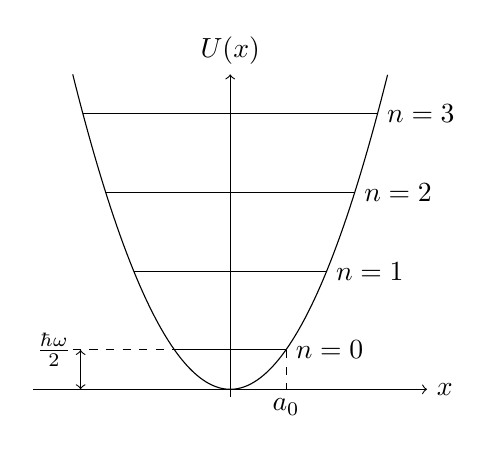
\begin{tikzpicture}[domain=-3.5:3.5]
   \draw[->] (-2.5,0) -- (2.5,0) node[right] {$x$};
  \draw[->] (0,-0.1) -- (0,4) node[above] {$U(x)$};
	\draw [domain=-2.0:2.0, samples=100] plot (\x, {\x*\x});
	\draw[dashed] (0.71,0.5) -- (0.71,0) node[below] {$a_0$};
	\draw[-] (-0.71,0.5) -- (0.71,0.5) node[right] {$n=0$};
	\draw[-] (-1.22,1.5) -- (1.22,1.5) node[right] {$n=1$};
	\draw[-] (-1.58,2.5) -- (1.58,2.5) node[right] {$n=2$};
	\draw[-] (-1.87,3.5) -- (1.87,3.5) node[right] {$n=3$};
  \draw[dashed] (-2, 0.5) -- (-0.71, 0.5);
  \draw[<->] (-1.9, 0) -- (-1.9, 0.5) node[left] {$\frac{\hbar \omega}{2}$};
  \end{tikzpicture}
\caption{Спектр гармонического осциллятора.} \label{fig:7_1}
\end{figure}


При $n = 0$:
$$
\frac{\hbar \omega}{2} = \frac{m\omega^2}{2} a_0^2  ~~\to~~ a_0 = \sqrt{\frac{\hbar}{m\omega}}
$$
-- амплитуда нулевых колебаний.

Из \eqref{eq:7_2_6}, \eqref{eq:7_2_9} и \eqref{eq:7_2_10}:
\begin{equation}
\label{eq:7_2_5_add}
\boxed {
	\cre\ket{n} = \sqrt{n+1}\ket{n+1}
}
\tag{\ref{eq:7_2_5}$'$}
\end{equation}

\begin{equation}
\label{eq:7_2_8_add}
\boxed {
	\ann\ket{n} = \sqrt{n}\ket{n-1}
}
\tag{\ref{eq:7_2_8}$'$}
\end{equation}

\section{Построение собственных функций осциллятора в координатном представлении с помощью операторов рождения и уничтожения. Связь $n$-го состояния осциллятора с основным.}

Введём обозначение: $\ket{0} \equiv \ket{\psi_0}$:
$$
\ann \ket{0} = 0 ~~~\text{или}~~~ \frac{1}{\sqrt{2}}(\op{\xi} + i\op{p_\xi}) \ket{\psi_0} = 0
$$

В $\xi$-представлении: $\op{p}_\xi = -i \D{}{\xi}$
$$
\brc{\xi + \D{}{\xi}} \psi_0(\xi) = 0
$$

Решение этого уравнения (волновая функция основного состояния гармонического осциллятора, нормированная на единицу):
$$
\boxed {
	\psi_0(\xi) = \frac{1}{\pi^{1/4}} e^{-\xi^2/2}
}
$$

\noindent
Обозначим $\ket{n} \equiv \ket{\psi_n}$

$$
\begin{gathered}
\cre \ket{0} = \sqrt{1} \ket{1} ~~~\to~~~ \ket{1} = \frac{1}{\sqrt{1}} \cre \ket{0} \\
\cre \ket{1} = \sqrt{2} \ket{2} ~~~\to~~~ \ket{2} = \frac{1}{\sqrt{2}} \cre \ket{1} = \frac{1}{\sqrt{2 \cdot 1}} (\cre)^2 \ket{0} \\
\cre \ket{2} = \sqrt{3} \ket{3} ~~~\to~~~ \ket{3} = \frac{1}{\sqrt{3}} \cre \ket{3} = \frac{1}{\sqrt{3 \cdot 2 \cdot 1}} (\cre)^3 \ket{0} \\
...
\end{gathered}
$$

$$
\boxed {
	\ket{\psi_n} \equiv \ket{n} = \sqrt{\frac{1}{n!}}(\cre)^n \ket{0}
}
$$

$$
\boxed {
	\psi_n(\xi) = \sqrt{\frac{1}{2^n \cdot n! \cdot \sqrt{\pi}}} \brc{\xi - \D{}{\xi}}^n e^{-\xi^2/2}
}
$$

Или через полиномы Эрмита:
$$
\boxed {
	\psi_n(\xi) = \sqrt{\frac{1}{2^n \cdot n! \cdot \sqrt{\pi}}} H_n(\xi) e^{-\xi^2/2}
}
$$
где $H_n(\xi) = e^{\xi^2/2} \brc{\xi - \D{}{\xi}}^n e^{-\xi^2/2} $

$$
H_0(\xi) = 1,~~ H_1(\xi) = 2\xi,~~ H_2(\xi) = 4\xi^2 - 2
$$
\begin{figure}[h]
  \centering
  \includegraphics[scale=0.3]{figs/7_2}
  \caption{Модуль волновых функций гармонического осциллятора}
  \label{fig:7_2}
\end{figure}

\begin{thm}[Осцилляторная теорема квантовой механики]
Волновая функция $\psi_n(x)$, соответствующая собственным значениям $E_n$, имеет при конечных $x$ ровно $n$ нулей.
\end{thm}
